% ch11-systems.tex -- Virtual memory
\chapter{Virtual memory: the address is a lie}
\label{ch:systems11}
\index{virtual memory}\index{page table}\index{TLB}\index{page fault}

Every address this book has used so far has been a polite fiction.
The pointer in your C program is not a DRAM address; it is a name in
a private namespace the OS maintains per process, translated on
every single load and store by hardware you never see. This chapter
opens that machinery: pages, the sv32 two-level walk, the TLB that
makes translation affordable, the page fault that makes demand
paging possible, and the protection bits that make processes safe
from each other --- all measured on the machine in front of you.

\section{Why virtualize}
\label{sec:why11}

Three problems one mechanism. \emph{Isolation}: process A cannot
scribble on process B because B's pages are simply absent from A's
map. \emph{Relocation}: every program may believe it owns address
\texttt{0x100000}; the OS places it anywhere. \emph{Sparse use}: a
program may reserve a gigabyte and touch a megabyte --- the rest
never needs to exist.

\begin{figure}[htbp]
\centering
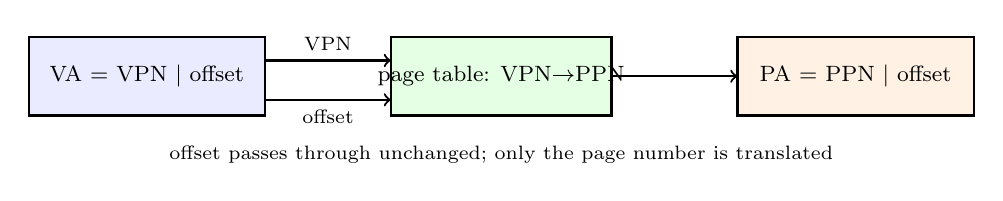
\begin{tikzpicture}[font=\footnotesize, x=1cm, y=1cm]
  \draw[thick, fill=blue!8] (0,2.4) rectangle (3,3.4);
  \node at (1.5,2.9) {VA = VPN $|$ offset};
  \draw[->,thick] (3,3.1) -- (4.6,3.1) node[midway,above]{\scriptsize VPN};
  \draw[->,thick] (3,2.6) -- (4.6,2.6) node[midway,below]{\scriptsize offset};
  \draw[thick, fill=green!10] (4.6,2.4) rectangle (7.4,3.4);
  \node at (6,2.9) {page table: VPN$\to$PPN};
  \draw[->,thick] (7.4,2.9) -- (9.0,2.9);
  \draw[thick, fill=orange!10] (9.0,2.4) rectangle (12,3.4);
  \node at (10.5,2.9) {PA = PPN $|$ offset};
  \node[font=\scriptsize] at (6,1.9) {offset passes through unchanged;
    only the page number is translated};
\end{tikzpicture}
\caption{Translation in one line: the virtual page number becomes a
physical page number through the page table; the offset rides along
untouched. Everything else --- TLBs, walks, faults --- is
engineering around this arrow.}
\label{fig:vapa11}
\end{figure}


\begin{example}[One line of truth]
Translation changes only the \emph{page number}; the offset inside
the page is identical on both sides. Everything in the chapter ---
the walk, the TLB, the fault path --- is machinery around that one
arrow.
\end{example}

\section{The walk: sv32 as the concrete case}
\label{sec:sv32_11}
\index{sv32}

RISC-V's 32-bit mode splits the VA into VPN[1] (10 bits), VPN[0]
(10 bits), offset (12 bits). VPN[1] indexes the level-1 page table
for the physical address of a level-0 table; VPN[0] indexes that for
the PPN. Two memory reads per translation.

\begin{figure}[htbp]
\centering
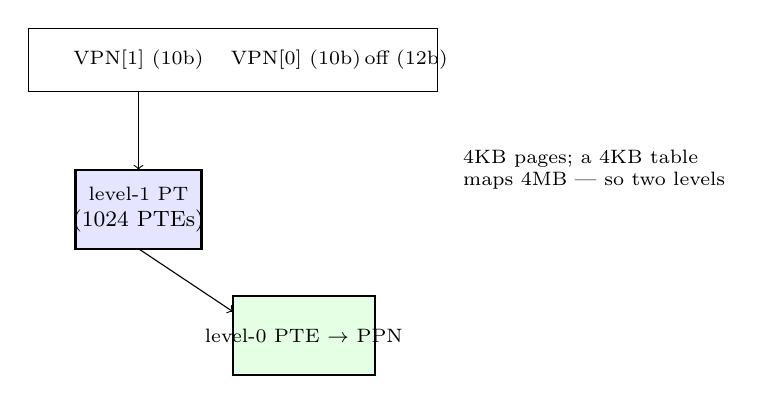
\begin{tikzpicture}[font=\footnotesize, x=1cm, y=1cm]
  \draw (0,3.6) rectangle (5.2,4.4);
  \node at (1.4,4.0) {\scriptsize VPN[1] (10b)};
  \node at (3.4,4.0) {\scriptsize VPN[0] (10b)};
  \node at (4.8,4.0) {\scriptsize off (12b)};
  \draw[->] (1.4,3.6) -- (1.4,2.6);
  \draw[thick,fill=blue!10] (0.6,1.6) rectangle (2.2,2.6);
  \node[align=center] at (1.4,2.1) {\scriptsize level-1 PT\\ (1024 PTEs)};
  \draw[->] (1.4,1.6) -- (2.6,0.8);
  \draw[thick,fill=green!10] (2.6,0.0) rectangle (4.4,1.0);
  \node at (3.5,0.5) {\scriptsize level-0 PTE $\to$ PPN};
  \node[anchor=west,align=left,font=\scriptsize] at (5.4,2.6)
    {4KB pages; a 4KB table\\ maps 4MB --- so two levels};
\end{tikzpicture}
\caption{The sv32 walk: VA[31:22] indexes the level-1 table for a
second-level table's physical address; VA[21:12] indexes that for
the PPN. Two memory reads per miss --- which is why the TLB exists.}
\label{fig:sv32_11}
\end{figure}


\begin{example}[A walk by hand]
VA \texttt{0x00401234}, satp pointing at a level-1 table at PPN
\texttt{0x1000}: VPN[1] = \texttt{0x001} $\to$ PTE at
\texttt{0x1000+1} gives level-0 table PPN \texttt{0x2000}; VPN[0] =
\texttt{0x001} $\to$ PTE at \texttt{0x2000+1} gives PPN
\texttt{0x9ABC}; PA = \texttt{0x9ABC} $|$ \texttt{0x234} =
\texttt{0x9ABC234}. Two lookups, one address.
\end{example}

\section{The TLB: caching the answer}
\label{sec:tlb11}

Two extra memory reads per load would be fatal. The TLB caches
VPN$\to$PPN results so that most accesses skip the walk entirely ---
it is a cache, exactly like ch10's, just for translations.

\begin{figure}[htbp]
\centering
\begin{tabular}{ll}
\toprule
stage & answers \\
\midrule
TLB lookup    & VPN$\to$PPN cached? (1 cycle-ish) \\
page-table walk & the real translation (2+ memory reads, sv32) \\
cache lookup  & PA $\to$ data (L1/L2/LLC) \\
DRAM          & last resort (our 120\,ns) \\
\bottomrule
\end{tabular}
\caption{The full chain every load traverses. A TLB hit collapses
the first two rows to almost nothing; a TLB miss costs the walk
\emph{plus} the data fetch --- translation and caching are two
separate caches strung in series.}
\label{fig:tlbchain11}
\end{figure}


\begin{example}[TLB reach]
A 64-entry TLB on 4\,KB pages covers 256\,KB of address space
before evictions start; on 2\,MB huge pages, 128\,MB. TLB reach is
why giant pages exist --- same hardware, 512$\times$ more coverage.
\end{example}

\section{Demand paging and the fault, measured}
\label{sec:fault11}

A page that is mapped but never touched may never exist. The first
touch raises a page fault; the OS allocates a frame, fills the PTE,
and retries the instruction. \texttt{ch11\_fault\_cost.c} mmaps
512\,MB and times the first walk vs.\ the second:

\begin{example}[The 7$\times$ first-touch tax, real]
\begin{verbatim}
pages=32768
first-touch 744 ns/page
resident    107.6 ns/page
fault cost 7x
\end{verbatim}
Verbatim: on 16\,KB pages, the fault costs 7$\times$ a resident
touch --- cheap enough that demand paging is the right lazy design,
expensive enough that when \emph{every} access faults (thrashing),
throughput collapses to disk speed.
\end{example}

\begin{figure}[htbp]
\centering
\begin{tabular}{lrr}
\toprule
access & Mac (16\,KB pages) & Linux container (4\,KB pages) \\
\midrule
resident page touch      & 107.6\,ns & 8.8\,ns \\
first touch (page fault) & 744\,ns   & 1101\,ns \\
\midrule
ratio                    & 7$\times$ & 125$\times$ \\
\bottomrule
\end{tabular}
\caption{\texttt{ch11\_fault\_cost.c}: mmap 512\,MB, touch one byte per
page twice. The fault costs roughly a microsecond on both machines. The
\emph{ratios} differ by a factor of 18 because the denominators do:
the Mac's ``resident'' touch is slow (each 16\,KB hop also misses the
cache), the container's is fast. Compare absolute times, not ratios.}
\label{fig:faultcurve11}
\end{figure}


\section{fork + copy-on-write, and the fence}
\label{sec:cow11}

\begin{figure}[htbp]
\centering
\begin{tabular}{lll}
\toprule
step & parent's page & child's page \\
\midrule
fork()        & shared, marked read-only & same frame \\
child writes  & fault $\to$ copy made    & private copy \\
parent writes & fault $\to$ copy made    & keeps sharing \\
\bottomrule
\end{tabular}
\caption{Copy-on-write: \texttt{fork} copies the page \emph{tables},
not the pages; the first \emph{write} to a shared page triggers the
fault that makes the copy. Measured in listing~\ref{lst:minflt11}: a child
that only reads 256 shared pages takes 0 faults, and one that then
writes them takes 256.}
\label{fig:cow11}
\end{figure}

\begin{figure}[htbp]
\centering
\begin{tabular}{lll}
\toprule
PTE bits & gate \\
\midrule
V (valid)   & present? else fault \\
R/W/X       & read / write / execute allowed? \\
U           & user-mode access allowed? \\
\bottomrule
\end{tabular}
\caption{The protection bits are the OS's fence, enforced by
hardware on every access. W$\wedge$X (never both) stops whole
classes of code-injection --- the bridge into Part IV's OS story.}
\label{fig:protect11}
\end{figure}


\begin{checkpoint}
Why can a shared library exist in every process at once? Same PPN
in many VPNs --- the page tables differ, the frames don't. Physical
memory is the shared resource; virtual memory is the private view.
\end{checkpoint}

\section{Common mistakes}
\label{sec:mistakes11}
\begin{itemize}
\item \textbf{Thinking VA $\approx$ PA is slow always.} With a TLB
      hit the translation is nearly free; the walk is the miss cost.
\item \textbf{Page size as a constant.} macOS arm64 uses 16\,KB;
      RISC-V sv32 uses 4\,KB; huge pages change TLB reach 512$\times$.
\item \textbf{A page fault is an error.} It is the load mechanism:
      mmap, COW, and lazy stack all run \emph{through} faults.
\item \textbf{Forgetting the fence is hardware.} PTE bits are
      checked on every access by the MMU --- protection isn't a
      convention, it's enforced.
\item \textbf{Thrashing as a cache problem.} It's a working-set
      problem: when the set exceeds resident frames, every level of
      the hierarchy stops mattering.
\end{itemize}

\section{Summary}
\label{sec:summary11}
\begin{tabularx}{\linewidth}{@{}l X@{}}
\toprule
\textbf{Piece} & \textbf{Measured/fixed version} \\
\midrule
pages     & VPN$\to$PPN, offset untouched \\
sv32 walk & 10+10+12 bits; two reads per miss \\
TLB       & translation cache; reach = entries $\times$ page size \\
fault     & 744\,ns vs 108\,ns resident on this machine (7$\times$) \\
COW       & fork = O(1); the first write pays \\
PTE bits  & V/R/W/X/U --- hardware-enforced fence \\
\bottomrule
\end{tabularx}

\section*{Further reading}
\label{sec:further11}
\begin{itemize}
\item Arpaci-Dusseau \& Arpaci-Dusseau, \emph{OSTEP} ch13--23 ---
      the ordering this chapter adapted:
      \url{https://pages.cs.wisc.edu/~remzi/OSTEP/}
\item CS:APP ch9 (VM + memory mapping):
      \url{https://csapp.cs.cmu.edu/}
\item xv6 book ch3 (page tables on real RISC-V code):
      \url{https://pdos.csail.mit.edu/6.828/2023/xv6/book-riscv-rev3.pdf}
\item RISC-V privileged spec, sv32 section:
      \url{https://riscv.org/specifications/}
\end{itemize}

\begin{rulebox}[Watch instead]
\begin{itemize}
\item \textbf{Virtual Memory --- Computerphile} --- pages and the
      walk at this chapter's altitude (verified 2026-10-11).
      \url{https://youtu.be/qdkxXygc3rE}
\end{itemize}
\end{rulebox}

\section*{Notes}
\label{sec:notes11}
\begin{itemize}
\item Fault/resident numbers are verbatim
      \texttt{ch11\_fault\_cost.c} on Apple Silicon (16\,KB pages);
      repeat on Linux to compare 4\,KB-page numbers.
\item COW is described, not run --- the chapter's trace table is a
      teaching aid; xv6 ch3 shows the real implementation.
\end{itemize}

\section*{Exercises}
\addcontentsline{toc}{section}{Exercises}
\stepcounter{section}

\begin{exercise}[easy]
A 32-bit VA has a 12-bit offset on sv32. How large is a page, and
how many pages fit in the VA space?
\end{exercise}
\begin{solution}[hint]
4\,KB; $2^{20}$ pages.
\end{solution}

\begin{exercise}[easy]
Which of isolation, relocation, sparse use does \emph{not} depend on
the page table being per-process?
\end{exercise}
\begin{solution}[hint]
Sparse use --- even a shared table could mark pages invalid.
\end{solution}

\begin{exercise}[easy]
TLB reach on 4\,KB pages with 64 entries vs 2\,MB huge pages with
the same 64 entries: compute both.
\end{exercise}
\begin{solution}[hint]
256\,KB vs 128\,MB.
\end{solution}

\begin{exercise}[medium]
Walk VA \texttt{0x00C02ABC} on sv32 by hand (level-1 table PPN
\texttt{0x4000}). Show both PTE indices.
\end{exercise}
\begin{solution}[hint]
VPN[1]=\texttt{0x003}, VPN[0]=\texttt{0x002}, off=\texttt{0xABC}.
\end{solution}

\begin{exercise}[medium]
Our fault measurement used anonymous mmap. Predict the first-touch
cost if the pages were file-backed, and name what changes.
\end{exercise}
\begin{solution}[hint]
Add disk I/O to the fault path --- $\mu$s scale, not ns.
\end{solution}

\begin{exercise}[medium]
Why must the TLB flush (or tag with ASIDs) on a context switch?
What breaks if it doesn't?
\end{exercise}
\begin{solution}[hint]
Process B inherits A's VPN$\to$PPN: silent cross-process aliasing.
\end{solution}

\begin{exercise}[medium]
Sketch the fork+COW trace for a parent that writes 10 shared pages
then reads 10: how many faults, and who pays them?
\end{exercise}
\begin{solution}[hint]
Parent pays all 10 write-faults; child's reads stay shared.
\end{solution}

\begin{exercise}[medium]
Design the experiment that separates TLB-miss cost from
page-fault cost on your machine. What do you stride over, and what
does the timing curve's knee reveal?
\end{exercise}
\begin{solution}[hint]
Stride one access per 4\,KB page over growing regions; the knee at
TLB reach shows walk cost.
\end{solution}

\begin{exercise}[hard]
Simulate CLOCK (second-chance) replacement vs LRU on a synthetic
10\,000-access trace with 50\% temporal reuse. Report hit rates for
both and explain the gap (or lack of one) from the algorithm
mechanics.
\end{exercise}
\begin{solution}[hint]
CLOCK approximates LRU well under temporal locality; gap widens on
scan workloads where LRU is fooled.
\end{solution}

\begin{exercise}[hard]
A system runs out of swap and the OOM killer picks the
\emph{wrong} process. Given only PTE protection bits and RSS
numbers, outline a policy that would have picked better, and its
cost.
\end{exercise}
\begin{solution}[hint]
Rank by frames-held$\times$last-touch-age; needs reference bits the
MMU already tracks --- cheap approximations exist.
\end{solution}

\begin{exercise}[hard]
Argue that W$\wedge$X (a page never writable \emph{and} executable)
cannot be defeated by any user-mode trick alone, then name the one
legitimate way JIT compilers still make code.
\end{exercise}
\begin{solution}[hint]
The fence is in the MMU, not the compiler; JITs map pages W first,
then \texttt{mprotect} to X --- never both.
\end{solution}
